\documentclass[10pt,a4paper,portrait]{article}

\usepackage[utf8]{inputenc}
\usepackage[a4paper,portrait,margin=0.6in,top=0.6in,bottom=0.6in]{geometry}
\usepackage{tikz}
\usetikzlibrary{shapes,arrows,positioning,calc,fit,backgrounds}
\usepackage{xcolor}
\usepackage{lmodern}
\usepackage{graphicx}

% =========================================================
% Palette & Styling (Minimal & Refined)
% =========================================================
\definecolor{primary}{RGB}{20, 42, 77}        % Rich Deep Navy
\definecolor{primarylight}{RGB}{30, 64, 115}   % Medium Navy
\definecolor{secondary}{RGB}{13, 148, 136}    % Deep Cyan/Teal
\definecolor{accentgold}{RGB}{217, 119, 6}     % Warm Amber/Gold
\definecolor{darkslate}{RGB}{30, 41, 59}      % Slate 800
\definecolor{mutedgray}{RGB}{100, 116, 139}   % Slate 500
\definecolor{cardbg}{RGB}{248, 250, 252}      % Soft Light Slate 50
\definecolor{cardborder}{RGB}{226, 232, 240}  % Crisp Border Line

\newcommand{\cmd}[1]{\texttt{#1}}

\begin{document}
\pagestyle{empty}

% =========================================================
% Subtle Minimal Frame
% =========================================================
\begin{tikzpicture}[remember picture, overlay]
  % Clean minimal outer border
  \draw[primary!25, line width=0.8pt, rounded corners=4pt] 
    ($(current page.north west)+(0.85cm, -0.85cm)$) rectangle ($(current page.south east)+(-0.85cm, 0.85cm)$);
\end{tikzpicture}

\vspace{0.4cm}

% =========================================================
% 1. University Logo & Department Header
% =========================================================
\begin{center}
  \IfFileExists{images/logo.png}{%
    
\includegraphics[height=2.35cm, keepaspectratio]{images/logo.png}
  }{%
    % Fallback Stylized Academic Crest
    
\begin{tikzpicture}[scale=0.90]
      \draw[primary, line width=1.6pt] (0,0) circle (1.40cm);
      \draw[secondary, line width=0.7pt, dashed] (0,0) circle (1.28cm);
      \draw[primary!30, line width=0.5pt] (0,0) circle (1.16cm);
      \fill[white] (0,0) circle (1.16cm);

      \foreach \ang in {130, 150, 170, 190, 210, 230} {
        \draw[secondary!80, fill=secondary!25, line width=0.4pt] 
          (\ang:0.95cm) ellipse (0.13cm and 0.05cm);
      }
      \foreach \ang in {50, 30, 10, -10, -30, -50} {
        \draw[secondary!80, fill=secondary!25, line width=0.4pt] 
          (\ang:0.95cm) ellipse (0.13cm and 0.05cm);
      }

      \draw[primary, fill=primary!8, line width=1.1pt, rounded corners=2pt]
        (-0.52, 0.52) -- (0.52, 0.52) -- (0.52, -0.06) arc(0:-180:0.52cm) -- cycle;
      
      \draw[primary, line width=1.1pt] (0, 0.44) -- (0, -0.38);
      \draw[secondary, line width=0.85pt] (-0.38, 0.30) to[bend left=15] (-0.06, 0.30);
      \draw[secondary, line width=0.85pt] (-0.38, 0.11) to[bend left=15] (-0.06, 0.11);
      \draw[secondary, line width=0.85pt] (-0.38, -0.08) to[bend left=15] (-0.08, -0.08);
      \draw[secondary, line width=0.85pt] (0.38, 0.30) to[bend right=15] (0.06, 0.30);
      \draw[secondary, line width=0.85pt] (0.38, 0.11) to[bend right=15] (0.06, 0.11);
      \draw[secondary, line width=0.85pt] (0.38, -0.08) to[bend right=15] (0.06, -0.08);

      \node[accentgold, font=\small] at (0, 0.76) {$\star$};
      \node[primary, font=\fontsize{4.8}{5.5}\selectfont\bfseries\sffamily] at (0, -0.80) {ESTD 2012};
    \end{tikzpicture}
  }

  \vspace{0.20cm}
  {\fontsize{19}{23}\selectfont\bfseries\sffamily\color{primary} KHWAJA YUNUS ALI UNIVERSITY\par}
  \vspace{0.07cm}
  {\fontsize{10.5}{13}\selectfont\bfseries\sffamily\color{secondary} DEPARTMENT OF COMPUTER SCIENCE AND ENGINEERING\par}
  
  \vspace{0.14cm}
  % Sleek Minimal Divider Line with Center Diamond
  
\begin{tikzpicture}
    \draw[primary!20, line width=0.6pt] (-4.5, 0) -- (4.5, 0);
    \draw[secondary, line width=1.4pt] (-1.8, 0) -- (1.8, 0);
    \draw[fill=primary, rotate=45] (-0.07, -0.07) rectangle (0.07, 0.07);
  \end{tikzpicture}
\end{center}

\vspace{0.18cm}

% =========================================================
% 2. Laboratory Report Badge & Course Info
% =========================================================
\begin{center}
  
\begin{tikzpicture}
    \node[
      fill=primary,
      text=white,
      font=\fontsize{10.5}{12.5}\selectfont\bfseries\sffamily,
      inner xsep=20pt,
      inner ysep=4.5pt,
      rounded corners=3pt
    ] {LABORATORY REPORT};
  \end{tikzpicture}

  \vspace{0.22cm}
  
\begin{tikzpicture}
    \node[
      draw=primary!20,
      fill=white,
      rounded corners=5pt,
      line width=0.7pt,
      inner xsep=18pt,
      inner ysep=6.5pt
    ] {
      \sffamily
      \textbf{\color{mutedgray}\small COURSE:} \textbf{\normalsize\color{primary} Operating System Lab} \quad
      \textcolor{primary!30}{\textbf{\textbar}} \quad
      \textbf{\color{mutedgray}\small CODE:} \textbf{\normalsize\color{secondary} CSE 0613-3104}
    };
  \end{tikzpicture}
\end{center}

\vspace{0.22cm}

% =========================================================
% 3. Experiment Title Card
% =========================================================
\begin{center}
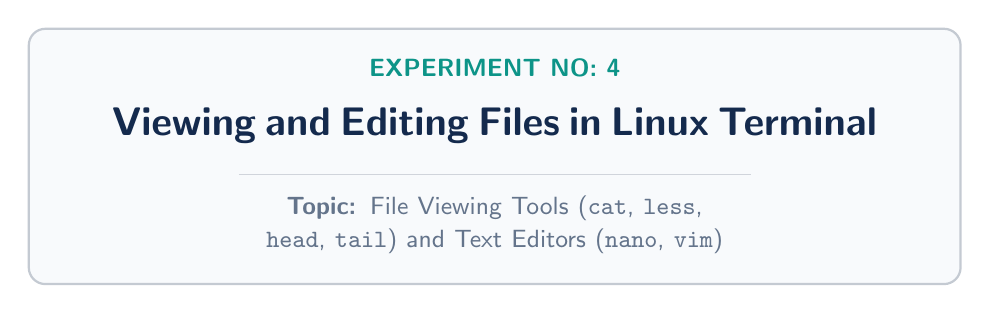
\begin{tikzpicture}
  \node[
    draw=primary!25,
    line width=0.8pt,
    fill=cardbg,
    rounded corners=6pt,
    inner xsep=20pt,
    inner ysep=11pt,
    text width=0.86\linewidth,
    align=center
  ] {
    {\color{secondary}\textbf{\sffamily\small EXPERIMENT NO: 4}}\par
    \vspace{0.14cm}
    {\fontsize{13.5}{17.5}\selectfont\bfseries\sffamily\color{primary}
    Viewing and Editing Files in Linux Terminal\par}
    \vspace{0.08cm}
    {\color{primary!20}\rule{6.5cm}{0.6pt}}\par
    \vspace{0.07cm}
    {\fontsize{9.5}{12}\selectfont\sffamily\color{mutedgray}
    \textbf{Topic:} File Viewing Tools (\texttt{cat}, \texttt{less}, \texttt{head}, \texttt{tail}) and Text Editors (\texttt{nano}, \texttt{vim})\par}
  };
\end{tikzpicture}
\end{center}

\vspace{0.18cm}

% =========================================================
% 4. Dates Bar
% =========================================================
\begin{center}

\begin{tikzpicture}
  \node[
    draw=cardborder,
    line width=0.6pt,
    fill=white,
    rounded corners=4pt,
    inner xsep=16pt,
    inner ysep=7pt,
    text width=0.86\linewidth
  ] {
    \begin{tabular*}{\linewidth}{@{\extracolsep{\fill}}lr@{}}
      \sffamily\small \textbf{\color{darkslate}Date of Experiment:} \hspace{0.2cm} \rule{3.8cm}{0.4pt} &
      \sffamily\small \textbf{\color{darkslate}Date of Submission:} \hspace{0.2cm} \rule{3.8cm}{0.4pt}
    \end{tabular*}
  };
\end{tikzpicture}
\end{center}

\vspace{0.22cm}

% =========================================================
% 5. Submitted By & Submitted To Cards
% =========================================================
\begin{center}
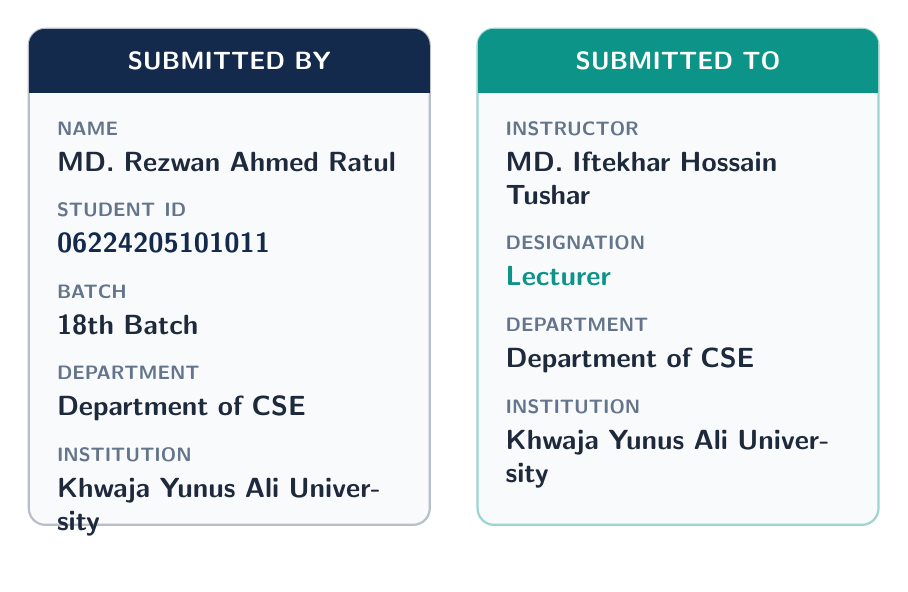
\begin{tikzpicture}
  % Card Dimensions
  \def\cardw{0.42\linewidth}
  \def\cardh{6.30cm}
  \def\headerh{0.82cm}

  % Card Left: Submitted By
  \coordinate (cl_topleft) at (0, 0);
  \coordinate (cl_botright) at (\cardw, -\cardh);
  
  \fill[cardbg, rounded corners=6pt] (cl_topleft) rectangle (cl_botright);
  \draw[primary!30, line width=0.8pt, rounded corners=6pt] (cl_topleft) rectangle (cl_botright);
  
  % Header Left
  \begin{scope}
    \clip[rounded corners=6pt] (cl_topleft) rectangle (cl_botright);
    \fill[primary] (cl_topleft) rectangle ($(cl_topleft)+(\cardw, -\headerh)$);
  \end{scope}
  \node[text=white, font=\sffamily\bfseries\small, anchor=center] at ($(cl_topleft)+(0.5*\cardw, -0.5*\headerh)$) {SUBMITTED BY};

  % Content Left
  \node[anchor=north west, inner sep=10pt, text width=\dimexpr\cardw-20pt\relax] at ($(cl_topleft)+(0, -\headerh)$) {
    {\sffamily\scriptsize\textbf{\color{mutedgray}NAME}}\par\vspace{1pt}
    {\sffamily\bfseries\fontsize{10}{12.5}\selectfont\color{darkslate} MD. Rezwan Ahmed Ratul}\par
    \vspace{4.5pt}
    {\sffamily\scriptsize\textbf{\color{mutedgray}STUDENT ID}}\par\vspace{1pt}
    {\sffamily\bfseries\color{primary} 06224205101011}\par
    \vspace{4.5pt}
    {\sffamily\scriptsize\textbf{\color{mutedgray}BATCH}}\par\vspace{1pt}
    {\sffamily\bfseries\color{darkslate} 18th Batch}\par
    \vspace{4.5pt}
    {\sffamily\scriptsize\textbf{\color{mutedgray}DEPARTMENT}}\par\vspace{1pt}
    {\sffamily\bfseries\color{darkslate} Department of CSE}\par
    \vspace{4.5pt}
    {\sffamily\scriptsize\textbf{\color{mutedgray}INSTITUTION}}\par\vspace{1pt}
    {\sffamily\bfseries\color{darkslate} Khwaja Yunus Ali University}\par
  };

  % Card Right: Submitted To
  \coordinate (cr_topleft) at (0.47\linewidth, 0);
  \coordinate (cr_botright) at ($(cr_topleft)+(\cardw, -\cardh)$);
  
  \fill[cardbg, rounded corners=6pt] (cr_topleft) rectangle (cr_botright);
  \draw[secondary!40, line width=0.8pt, rounded corners=6pt] (cr_topleft) rectangle (cr_botright);
  
  % Header Right
  \begin{scope}
    \clip[rounded corners=6pt] (cr_topleft) rectangle (cr_botright);
    \fill[secondary] (cr_topleft) rectangle ($(cr_topleft)+(\cardw, -\headerh)$);
  \end{scope}
  \node[text=white, font=\sffamily\bfseries\small, anchor=center] at ($(cr_topleft)+(0.5*\cardw, -0.5*\headerh)$) {SUBMITTED TO};

  % Content Right
  \node[anchor=north west, inner sep=10pt, text width=\dimexpr\cardw-20pt\relax] at ($(cr_topleft)+(0, -\headerh)$) {
    {\sffamily\scriptsize\textbf{\color{mutedgray}INSTRUCTOR}}\par\vspace{1pt}
    {\sffamily\bfseries\fontsize{10}{12.5}\selectfont\color{darkslate} MD. Iftekhar Hossain Tushar}\par
    \vspace{4.5pt}
    {\sffamily\scriptsize\textbf{\color{mutedgray}DESIGNATION}}\par\vspace{1pt}
    {\sffamily\bfseries\color{secondary} Lecturer}\par
    \vspace{4.5pt}
    {\sffamily\scriptsize\textbf{\color{mutedgray}DEPARTMENT}}\par\vspace{1pt}
    {\sffamily\bfseries\color{darkslate} Department of CSE}\par
    \vspace{4.5pt}
    {\sffamily\scriptsize\textbf{\color{mutedgray}INSTITUTION}}\par\vspace{1pt}
    {\sffamily\bfseries\color{darkslate} Khwaja Yunus Ali University}\par
  };
\end{tikzpicture}
\end{center}

\vfill

% =========================================================
% 6. Instructor's Signature & Date
% =========================================================
\begin{center}

\begin{tikzpicture}
  \node[
    draw=primary!20,
    line width=0.7pt,
    fill=white,
    rounded corners=5pt,
    inner xsep=16pt,
    inner ysep=9pt,
    text width=0.86\linewidth
  ] {
    \begin{tabular*}{\linewidth}{@{\extracolsep{\fill}}lr@{}}
      \begin{tabular}{@{}l@{}}
        \textbf{\sffamily\small\color{darkslate} Remarks / Evaluation:}\\[12pt]
        \rule{5.2cm}{0.4pt}
      \end{tabular} &
      \begin{tabular}{@{}c@{}}
        \vspace{12pt}\null\\
        \rule{5.6cm}{0.5pt}\\[3pt]
        \textbf{\sffamily\small\color{primary} Instructor's Signature \& Date}
      \end{tabular}
    \end{tabular*}
  };
\end{tikzpicture}
\end{center}

\vspace{0.25cm}

\end{document}
